\documentclass[aspectratio=169,svgnames,dvipsnames]{beamer}
% \beamertemplatenavigationsymbolsempty{}
% \setbeamertemplate{footline}[frame number]

\usepackage{mathtools}
\usepackage{mathpazo}
\usepackage{newpxmath}
\usepackage{newpxtext}
\usepackage[T1,small,euler-digits]{eulervm}
% \usecolortheme[named=Maroon]{structure}
% \beamertemplatesolidbackgroundcolor{Snow}

\usepackage{siunitx}
\usepackage{makecell, booktabs, caption}
\usepackage{multirow}
\usepackage{tabularx}
\usepackage{listings}
\usepackage{tcolorbox}

\definecolor{darkmagenta}{rgb}{0.55, 0.0, 0.55}
\definecolor{fulvous}{rgb}{0.86, 0.52, 0.0}
\definecolor{ginger}{rgb}{0.69, 0.4, 0.0}
\definecolor{lavenderindigo}{rgb}{0.58, 0.34, 0.92}
\definecolor{bluegray}{rgb}{0.4, 0.6, 0.8}
\definecolor{myBlue}{RGB}{0,0,255}
\definecolor{myPurple}{RGB}{128,0,128}
\definecolor{myOrange}{RGB}{255,165,0}
\definecolor{myTeal}{RGB}{0,128,128}
\definecolor{myBrown}{RGB}{139,69,19}

\newcommand{\colorA}{myBlue}
\newcommand{\colorB}{myPurple}
\newcommand{\colorC}{myOrange}
\newcommand{\colorD}{myTeal}
\newcommand{\colorE}{myBrown}

\usetheme{default}

\newcommand\blfootnote[1]{%
  \begingroup
  \renewcommand\thefootnote{}\footnote{#1}%
  \addtocounter{footnote}{-1}%
  \endgroup
}
\setbeamertemplate{navigation symbols}{
    \usebeamerfont{footline}
    \footnotesize
    \color{black}
    \hspace{1em}\insertframenumber
}
\usecolortheme{spruce}
\setbeamertemplate{headline}{}

\newcommand\hmmax{0}
\newcommand\bmmax{0}

\newenvironment{changemargin}[2]{%
\begin{list}{}{%
\setlength{\topsep}{0pt}%
\setlength{\leftmargin}{#1}%
\setlength{\rightmargin}{#2}%
\setlength{\listparindent}{\parindent}%
\setlength{\itemindent}{\parindent}%
\setlength{\parsep}{\parskip}%
}%
\item[]}{\end{list}}

\newcommand{\myframe}[1]
{
{
\setbeamercolor{background canvas}{bg=black}
\color{white}
\begin{frame}{}{}
  \begin{changemargin}{-1cm}{-1cm}
  \Huge
  \centering
  #1
  \end{changemargin}
\end{frame}
}
}

\newcommand\Wider[2][5em]{%
\makebox[\linewidth][c]{%
  \begin{minipage}{\dimexpr\textwidth+#1\relax}
  \raggedright#2
  \end{minipage}%
  }%
}

\newcommand<>{\oncolor}[2]{%
  \alt#3{\textcolor{#1}{#2}}{#2}%
}

\title{KATch: A Fast Symbolic Verifier for NetKAT}
% \subtitle{(POPL'23)}
\date{}

\newcommand{\td}[1]{\textbf{\color{orange}#1\color{orange}}}
\newcommand{\RED}[1]{\textbf{\color{red}#1\color{black}}}
\newcommand{\GREEN}[1]{\textbf{\color{ForestGreen}#1\color{black}}}
\newcommand{\MAROON}[1]{\textbf{\color{Maroon}#1\color{black}}}


% =========== TIKZ ===========
\usepackage{graphicx}
\usepackage{tikz}
\usetikzlibrary{shapes.geometric, arrows}
\usetikzlibrary{fit}
\usetikzlibrary{svg.path}
% \usetikzlibrary{graphdrawing}
% \usetikzlibrary{graphdrawing.force}
% \usetikzlibrary{graphdrawing.layered}
\usetikzlibrary{decorations}
\usetikzlibrary{decorations.markings}
\usetikzlibrary{backgrounds}
\usetikzlibrary{tikzmark}


\newif\ifshowtikz
\showtikztrue
% \showtikzfalse   % <---- comment/uncomment that line

\let\oldtikzpicture\tikzpicture
\let\oldendtikzpicture\endtikzpicture

\renewenvironment{tikzpicture}{%
    \ifshowtikz\expandafter\oldtikzpicture%
    \else\comment%
    \fi
}{%
    \ifshowtikz\oldendtikzpicture%
    \else\endcomment%
    \fi
}

\raggedbottom

% =============================

\newcommand{\bigsep}{\mathop{\scalebox{1.5}{\raisebox{-0.2ex}{$\sep$}}}}%

\newcommand{\ie}{\textit{i.e.,}\ }
\newcommand{\eg}{\textit{e.g.,}\ }
\newcommand{\etc}{\textit{etc.}\ }
\newcommand{\viceversa}{\textit{vice versa}}
\newcommand{\wrt}{w.r.t.\ }


\newcommand{\Bit}{\{0,1\}}

\newcommand{\codeblock}[1]{
  \begin{array}[t]{@{} l}
    #1
  \end{array}
}
\newcommand{\codeblockc}[1]{
  \begin{array}{@{} l}
    #1
  \end{array}
}

% Base language

\newcommand{\keyword}[1]{\mathbf{#1}}
\newcommand{\lam}[1]{\lambda #1.\ }
\newcommand{\letS}[1]{\keyword{let}\ #1\ =\ }
\newcommand{\inS}{\ \keyword{in}\ }

\newcommand{\unitV}{()}
\newcommand{\inXS}[1]{\keyword{in_{#1}}}
\newcommand{\inleftS}{\inXS{L}}
\newcommand{\inrightS}{\inXS{R}}
\newcommand{\inleft}[1]{\inleftS(#1)}
\newcommand{\inright}[1]{\inrightS(#1)}
\newcommand{\inX}[2]{\inXS{#1}(#2)}
\newcommand{\matchwith}[2]{\keyword{match}\ #1\ \keyword{with}\ #2\ \keyword{end}}
\newcommand{\matchclause}[2]{#1 \Rightarrow #2}
\newcommand{\matchempty}[1]{\matchwith{#1}{\bot}}

\newcommand{\fork}{\keyword{fork}}
\newcommand{\some}{\keyword{Some}}
\newcommand{\none}{\keyword{None}}

\newcommand{\voidT}{\keyword{0}}
\newcommand{\unitT}{\keyword{1}}
\newcommand{\funT}{\mathrel{-\kern-1pt\circ}}


% Binary sessions

\newcommand{\Session}{\textdom{Session}}
\newcommand{\session}{s}
\newcommand{\chan}{c}

\newcommand{\Bfork}{\keyword{fork_C}}
\newcommand{\Bsend}{\keyword{send_C}}
\newcommand{\Brecv}{\keyword{receive_C}}
\newcommand{\Bclose}{\keyword{close_C}}
\newcommand{\Bwait}{\keyword{wait_C}}
\newcommand{\BtellL}{\keyword{tell_L}}
\newcommand{\BtellR}{\keyword{tell_R}}
\newcommand{\Bask}{\keyword{ask}}


\newcommand{\BsendT}{\text{\textbf{!}}}
\newcommand{\BrecvT}{\text{\textbf{?}}}
\newcommand{\BendT}{\keyword{End}}
\newcommand{\BendTS}{\mathsf{End_{\text{\textbf{!}}}}}
\newcommand{\BendTR}{\mathsf{End_{\text{\textbf{?}}}}}
\DeclareMathOperator{\BtellT}{\keyword{\&}}
\DeclareMathOperator{\BaskT}{\keyword{\oplus}}


% Locks
\newcommand{\lock}{\ell}
\newcommand{\Lnew}{\keyword{new}}
\newcommand{\Lacquire}{\keyword{acquire}}
\newcommand{\Lrelease}{\keyword{release}}
\newcommand{\Ldrop}{\keyword{drop}}
\newcommand{\Lwait}{\keyword{wait}}
\newcommand{\Lfork}{\keyword{fork}}

% \newcommand{\LlockT}[3]{\keyword{Lock}\langle {#3}{\,}^{#1}_{#2} \rangle}
\newcommand{\LlockT}[3]{\langle {#3}{\,}^{#1}_{#2} \rangle}
\newcommand{\Lownership}{a}
\newcommand{\Lowner}{1}
\newcommand{\Lclient}{0}
\newcommand{\Lstate}{b}
\newcommand{\Lopened}{1}
\newcommand{\Lclosed}{0}
% \newcommand{\Lcapsplit}[3]{\keyword{locksplit}\ #1\ #2\ #3}

% Lock groups

% \newcommand{\LGnewgroup}{\keyword{newgroup_G}}
% \newcommand{\LGdropgroup}{\keyword{dropgroup_G}}
% \newcommand{\LGnew}[1]{\keyword{newlock_G}[#1]}
% \newcommand{\LGacquire}[1]{\keyword{acquire_G}[#1]}
% \newcommand{\LGrelease}[1]{\keyword{release_G}[#1]}
% \newcommand{\LGdrop}[1]{\keyword{droplock_G}[#1]}
% \newcommand{\LGwait}[1]{\keyword{wait_G}[#1]}
% \newcommand{\LGfork}{\keyword{fork_G}}

\newcommand{\LGnewgroup}{\keyword{newgroup}}
\newcommand{\LGdropgroup}{\keyword{dropgroup}}
\newcommand{\LGnew}[1]{\keyword{new}[#1]}
\newcommand{\LGacquire}[1]{\keyword{acquire}[#1]}
\newcommand{\LGrelease}[1]{\keyword{release}[#1]}
\newcommand{\LGdrop}[1]{\keyword{drop}[#1]}
\newcommand{\LGwait}[1]{\keyword{wait}[#1]}
\newcommand{\LGfork}{\keyword{fork}}

% \newcommand{\LGlockgroupT}[1]{\keyword{Lock_G}\langle #1 \rangle}
% \newcommand{\LGlockgroupT}[1]{\keyword{Lock}\langle #1 \rangle}
\newcommand{\LGlockgroupT}[1]{\langle #1 \rangle}
\newcommand{\LGvec}{\vec{g}}
\newcommand{\LGlock}[3]{{#3}{}^{#1}_{#2}}
\newcommand{\LGcapsplit}[3]{\keyword{split}\ #1\ \keyword{into}\ #2,#3}

\newcommand{\LGlen}[1]{|{#1}|}
\newcommand{\LGallclosed}[1]{\keyword{closed}\ #1}
\newcommand{\LGallowners}[1]{\keyword{owners}\ #1}


% Typing rules
\newcommand{\envsplit}[3]{\keyword{split}\ #1\ #2\ #3}
\newcommand{\typed}[3]{#1 \vdash #2 : #3}
\newcommand{\typedz}[2]{#1\! :\! #2}
\newcommand{\ctx}{\Gamma}
\newcommand{\ctxdisjoint}{\mathrel{\bot}}
\newcommand{\ctxsplit}[3]{#1 \equiv #2 \cdot #3}
\newcommand{\ctxsplitS}{\ctxsplit {\ctx} {\ctx_1} {\ctx_2}}
\newcommand{\unrestricted}[1]{#1\ \mathsf{unr}}


\newcommand{\Type}{\keyword{Type}}
\newcommand{\type}{\tau}

% Operational semantics

\newcommand{\istep}[1]{\overset{#1}{\leadsto}}
\newcommand{\pstep}{\leadsto_\mathrm{pure}}

\newcommand{\Cfg}{\mathsf{Cfg}}
\newcommand{\cfg}{\rho}

\newcommand{\ThreadV}{\mathsf{Thread}}
\newcommand{\BarrierV}{\mathsf{Barrier}}
\newcommand{\SessionV}{\mathsf{Session}}
\newcommand{\LockV}{\mathsf{Lock}}

\newcommand{\locklit}[1]{\left< #1 \right>}
\newcommand{\lockGlit}[2]{\left< #1 \mid #2\right>}
\newcommand{\refcnt}{\mathsf{refcnt}}
\newcommand{\lockopt}{x}

% Theorems / proof

\newcommand{\waiting}{\ \mathsf{waiting}_\cfg\ }
\newcommand{\blocked}{\ \mathsf{blocked}\ }
\newcommand{\cfgrefs}{\mathsf{refs}_{\cfg}}
\newcommand{\inv}{\mathsf{inv}}


% \renewcommand{\step}{\leadsto}
% \newcommand{\steps}{\step^*}
% \newcommand{\hstep}{\leadsto_\mathrm{head}}
% \newcommand{\lstep}{\leadsto_\mathrm{local}}
% \newcommand{\istep}[1]{\overset{#1}{\leadsto}}
% \newcommand{\gstep}{\leadsto_\mathrm{cfg}}
% \newcommand{\append}{+\kern-1ex+\kern0.8ex}
% \newcommand{\length}[1]{| #1 |}
% \newcommand{\blockedShort}[1]{\mathsf{blocked}_{#1}}
% \newcommand{\blocked}[3][]{\blockedShort{#1}(#2, #3)}

\setlength\arraycolsep{1pt}

\newcommand{\config}[1]{
  \begin{Bmatrix*}[l]
    #1
  \end{Bmatrix*}
}

\usepackage{xspace}
\newcommand{\KATch}{KATch\xspace}
\newcommand{\Frenetic}{\textsc{Frenetic}\xspace}

% Define custom colors
\definecolor{frametitlefg}{HTML}{1b3f41}
\definecolor{frametitlebg}{HTML}{d4eced}
\setbeamercolor{frametitle}{bg=frametitlebg, fg=frametitlefg}
\definecolor{titleslidebackground}{rgb}{1, 1, 0.949}

\setbeamertemplate{itemize items}[circle]
\setbeamercolor{itemize item}{fg=frametitlefg!70}


\begin{document}

{
\setbeamercolor{background canvas}{bg=titleslidebackground}
\begin{frame}
  % \vspace{0.5cm}
  % \titlepage{}
  % \vspace{-2cm}
  % \begin{minipage}[t]{0.50\textwidth}
  %   \begin{center}
  %     \textbf{Jules Jacobs} \\[4pt]
  %     \scriptsize Radboud University
  %     $\to$
  %     \scriptsize Cornell University
  %   \end{center}
  % \end{minipage}
  % \begin{minipage}[t]{0.40\textwidth}
  %   \begin{center}
  %     \textbf{Stephanie Balzer} \\[4pt]
  %     \scriptsize Carnegie Mellon University
  %   \end{center}
  % \end{minipage}
  % \vspace{0.6cm}

  % \vspace{0.8cm}
  \centering
  
\includegraphics[scale=0.15]{katch2.png}\\[-3mm]
  \huge \textbf{KATch}\\[-0.8em]
  \rule{5cm}{1pt}

  \Large A Fast Symbolic Verifier for NetKAT
  % 
\includegraphics[scale=0.33]{deriv/deriv.pdf}
  % 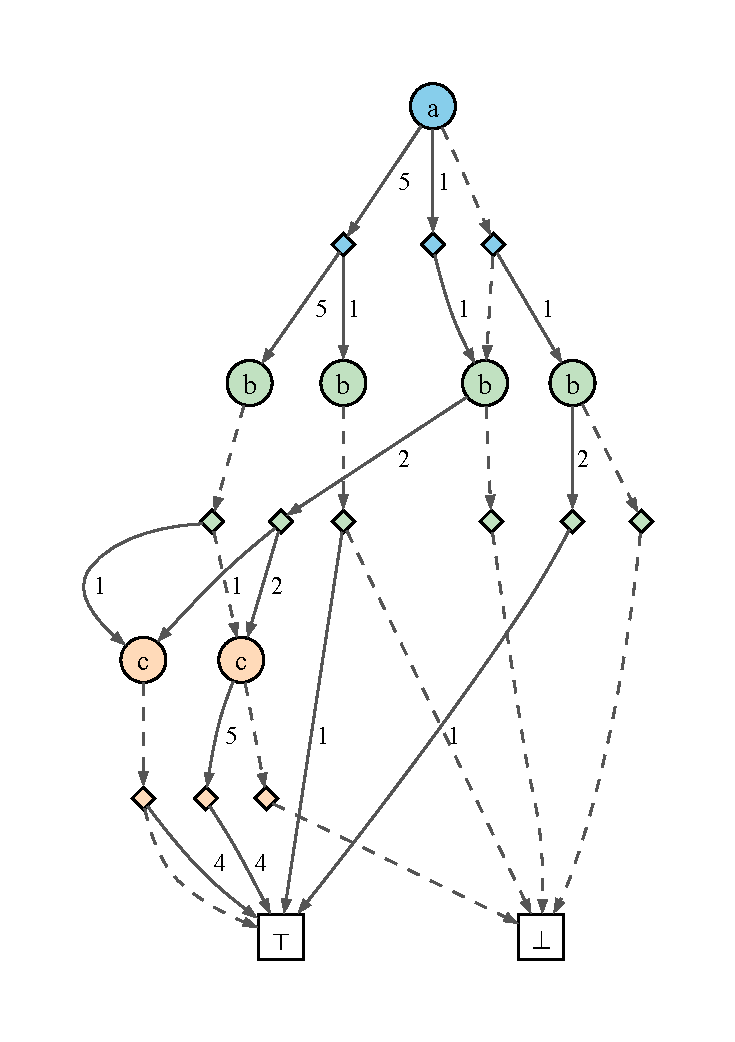
\includegraphics[scale=0.3]{viz/spp1seq2.pdf}
  \vspace{0.5cm}

  \small
  Mark Moeller, Jules Jacobs, Nate Foster, Alexandra Silva (Cornell),
  Olivier Savary Belanger, David Darais, Cole Schlesinger (Galois),
  Steffen Smolka (Google)
\end{frame}
}

\begin{frame}
  \frametitle{The Control Plane and Network Defense Agents}

  \begin{columns}[t]
      \begin{column}{0.45\textwidth}
          \textbf{Control Plane}
          \begin{itemize}
              \item Computes routing tables
              \item Ensures network connectivity
              \item Enforces network policies
          \end{itemize}
      \end{column}

      \begin{column}{0.55\textwidth}
          \textbf{Network Defense Agents}
          \begin{itemize}
              \item Detects and responds to network attacks
              \item Example: Security breach containment
              \item Example: DDoS mitigation
              \item \textbf{Action space?}
              \item \textbf{Modify routing tables?}
          \end{itemize}
      \end{column}
  \end{columns}

\end{frame}

\begin{frame}
  \frametitle{Neural and Symbolic AI}

  \begin{columns}[t]
      \begin{column}{0.5\textwidth}
          \textbf{Neural Strengths}
          \begin{itemize}
              \item General pattern recognition
              \item Learns from experience
              \item Adaptability to new situations
              \item Ideal when explicit programming is difficult
          \end{itemize}
      \end{column}

      \begin{column}{0.5\textwidth}
          \textbf{Symbolic Strengths}
          \begin{itemize}
              \item Domain specific reasoning
              \item Guarantees correctness
              \item Verifiable and explainable
              \item Ideal when strict compliance with rules is required
          \end{itemize}
      \end{column}
  \end{columns}

\end{frame}

\begin{frame}
  \frametitle{Neural+Symbolic AI in Network Defense: Idea}

  \begin{columns}[t]
      \begin{column}{0.5\textwidth}
          \textbf{Neural}
          \begin{itemize}
              \item Utilizes deep learning for real-time attack detection and response
              \item Adapts to evolving network threats
              \item Modifies routing tables dynamically
              \item Example: Detecting and rerouting traffic to mitigate DDoS attacks
              \item Example: Detecting and isolating compromised hosts
          \end{itemize}
      \end{column}

      \begin{column}{0.5\textwidth}
          \textbf{Symbolic}
          \begin{itemize}
              \item Computes consequences of routing changes
              \item Ensures correctness of routing tables
              \item Verifies adherence to network policies and security rules
              \item Example: Validating routing paths for security compliance
              \item Example: Verifying reachability of critical network services
          \end{itemize}
      \end{column}
  \end{columns}

\end{frame}

\begin{frame}
  \frametitle{NetKAT: Symbolic Network Reasoning}

  \textbf{NetKAT: network specification language for SDN}
  \begin{itemize}
    \item Network topology
    \item Routing tables
    \item Network-wide policies
  \end{itemize}

  \medskip
  \textbf{Verification of network policies}
  \begin{itemize}
    \item Security properties, e.g. slice isolation
    \item Operational properties, e.g. reachability
    \item Verified in a common framework
  \end{itemize}

  \bigskip

  \textbf{Problem: } NetKAT verification is slow\\
  Not suitable for real-time network defense\\[5mm]

\end{frame}

{
\setbeamercolor{background canvas}{bg=titleslidebackground}
\begin{frame}
  % \vspace{0.8cm}
  \centering
  
\includegraphics[scale=0.15]{katch2.png}\\[-3mm]
  \huge \textbf{KATch}\\[-0.8em]
  \rule{5cm}{1pt}

  \Large A Fast Symbolic Verifier for NetKAT
  % 
\includegraphics[scale=0.33]{deriv/deriv.pdf}
  % 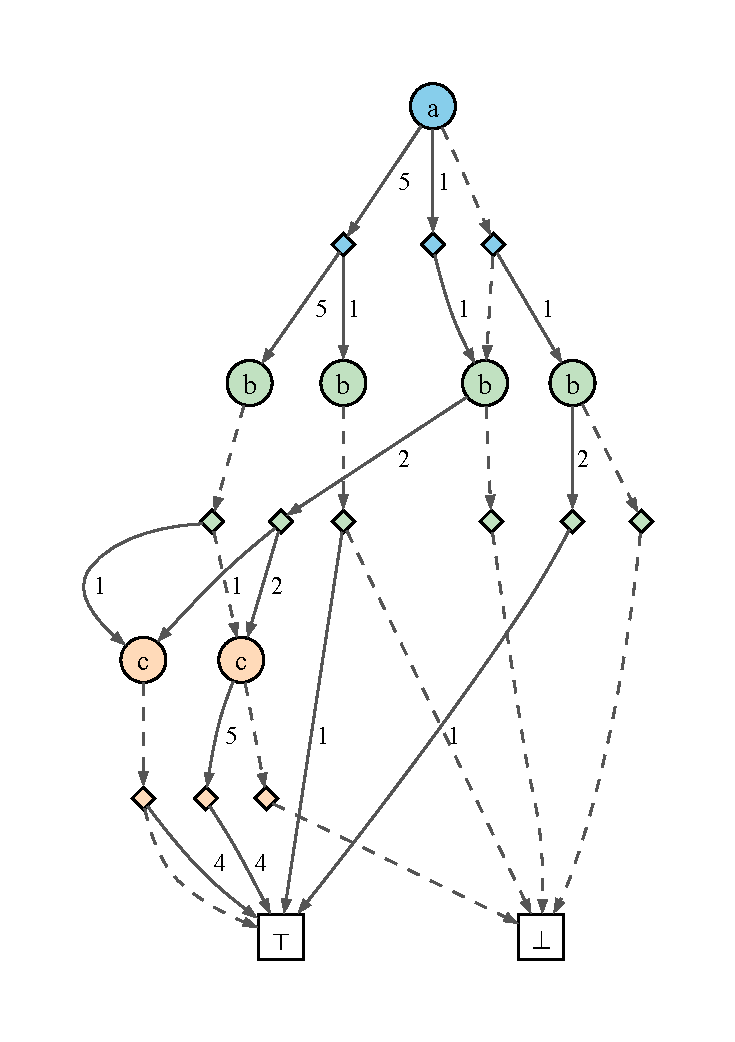
\includegraphics[scale=0.3]{viz/spp1seq2.pdf}
  \vspace{0.5cm}
\end{frame}
}

\begin{frame}
  \frametitle{KATch}

  A new NetKAT verifier that is
  \begin{itemize}
    \item \textbf{Fast:} 1000$\times$ faster
    \item \textbf{Symbolic:} explains verification failures
    \item \textbf{Scalable:} handles larger networks
  \end{itemize}
\end{frame}

\begin{frame}
  \frametitle{Full Reachability}
  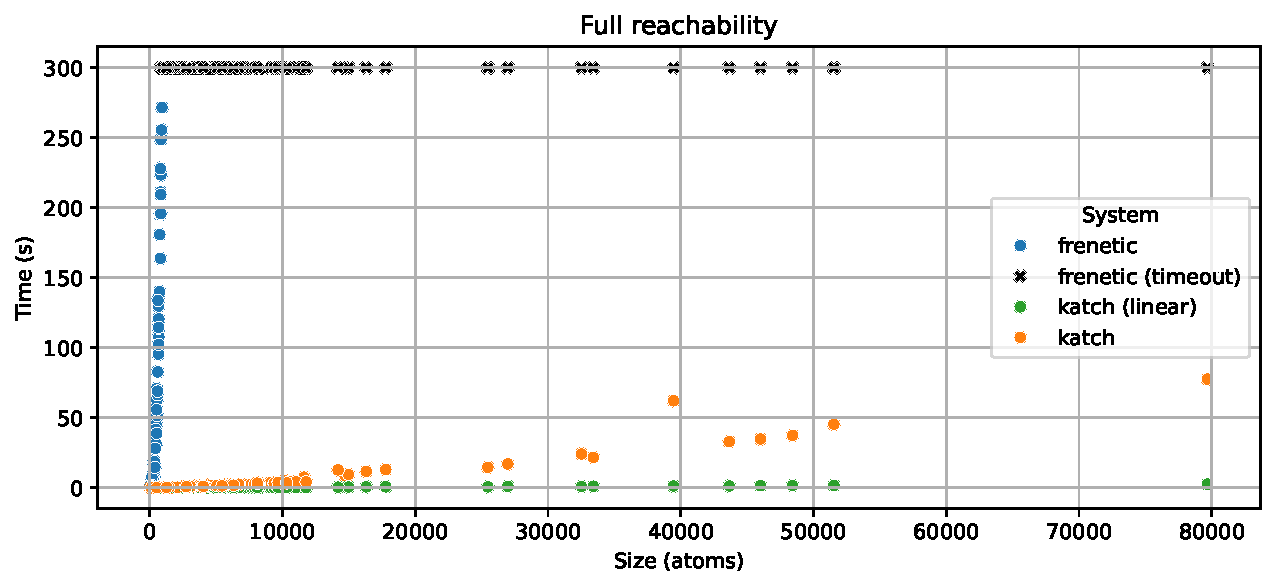
\includegraphics[scale=0.6]{plots/Full reachability_time_vs_size_wide.pdf}
\end{frame}

\begin{frame}
  \frametitle{Detailed comparison: (un)reachability and slice isolation}
  \scalebox{0.85}{\begin{tabular}{llrrr}
\toprule
name & type & Size (KB) & KATch (s) & Frenetic (s) \\
\midrule
Layer42 & unreachability & 1.59 & 0.00 & 0.04 \\
Layer42 & reachability & 1.60 & 0.00 & 0.04 \\
Layer42 & slicing & 1.71 & 0.01 & 0.07 \\
Compuserv & unreachability & 5.94 & 0.01 & 0.38 \\
Compuserv & reachability & 5.95 & 0.01 & 0.36 \\
Compuserv & slicing & 6.16 & 0.01 & 0.85 \\
Airtel & unreachability & 8.67 & 0.01 & 0.84 \\
Airtel & reachability & 8.68 & 0.01 & 0.83 \\
Airtel & slicing & 8.86 & 0.02 & 2.08 \\
Belnet & unreachability & 15.21 & 0.01 & 3.16 \\
Belnet & reachability & 15.22 & 0.01 & 3.17 \\
Belnet & slicing & 15.55 & 0.04 & 7.99 \\
Shentel & unreachability & 20.42 & 0.02 & 4.00 \\
Shentel & reachability & 20.43 & 0.02 & 4.01 \\
Shentel & slicing & 20.82 & 0.04 & 9.80 \\
Arpa & unreachability & 21.50 & 0.02 & 4.32 \\
Arpa & reachability & 21.51 & 0.01 & 4.32 \\
Arpa & slicing & 21.91 & 0.05 & 10.99 \\
ft4 & reachability & 30.16 & 0.02 & 2.27 \\
ft4 & slicing & 30.20 & 0.03 & 5.53 \\
ft4 & reachability & 32.41 & 0.02 & 10.51 \\
Sanet & unreachability & 44.90 & 0.03 & 25.23 \\
Sanet & reachability & 44.91 & 0.04 & 23.46 \\
Sanet & slicing & 45.49 & 0.12 & 62.70 \\
Uunet & unreachability & 59.77 & 0.04 & 81.92 \\
Uunet & reachability & 59.78 & 0.04 & 81.54 \\
Uunet & slicing & 60.45 & 0.15 & 204.85 \\
Missouri & unreachability & 106.11 & 0.10 & 165.85 \\
Missouri & reachability & 106.12 & 0.11 & 161.28 \\
Missouri & slicing & 107.02 & 0.27 & 519.46 \\
Telcove & unreachability & 117.62 & 0.08 & 465.27 \\
Telcove & reachability & 117.64 & 0.09 & 464.15 \\
Telcove & slicing & 118.58 & 0.28 & 1274.24 \\
ft6 & reachability & 228.16 & 0.25 & 1033.57 \\
ft6 & reachability & 250.33 & 0.12 & 259.80 \\
ft6 & slicing & 250.37 & 0.35 & 793.83 \\
Deltacom & unreachability & 297.62 & 0.30 & 2523.03 \\
Deltacom & reachability & 297.63 & 0.31 & 2392.56 \\
Deltacom & slicing & 299.14 & 0.75 & 5334.77 \\
ft8 & unreachability & 649.58 & 0.77 & 10026.25 \\
ft8 & reachability & 649.60 & 0.67 & 9292.22 \\
Cogentco & reachability & 894.96 & 0.97 & 13090.69 \\
Cogentco & unreachability & 894.96 & 0.88 & 13450.43 \\
\bottomrule
\end{tabular}
}
\end{frame}

\begin{frame}
  \frametitle{Synthetic combinatorial benchmarks}

  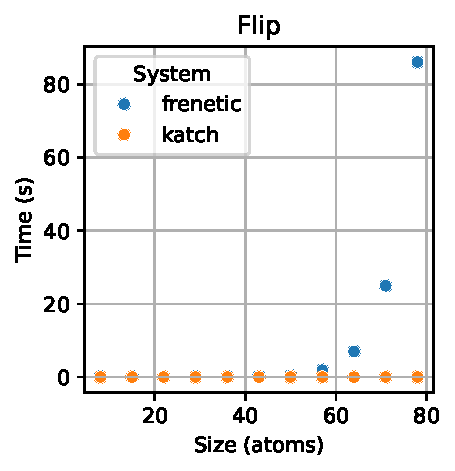
\includegraphics[scale=0.53]{plots/Flip_time_vs_size.pdf}
  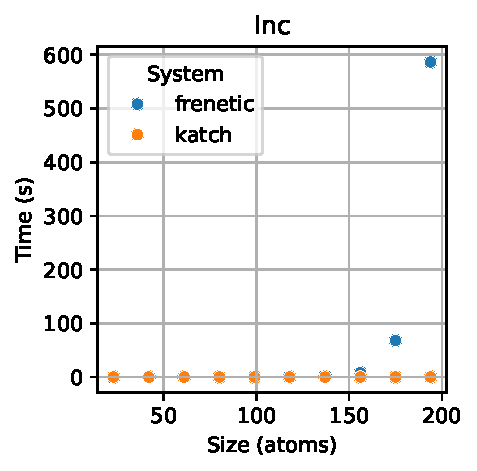
\includegraphics[scale=0.53]{plots/Inc_time_vs_size.pdf}
  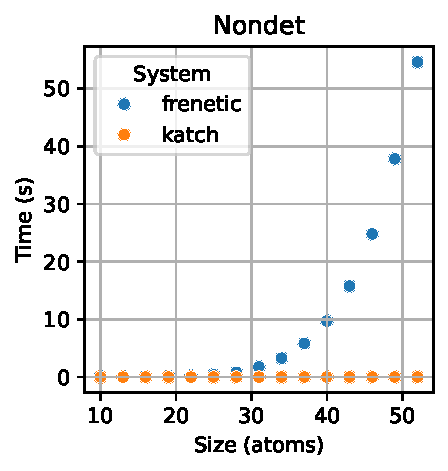
\includegraphics[scale=0.53]{plots/Nondet_time_vs_size.pdf}
\end{frame}

\begin{frame}
  \frametitle{Conclusion}

  \textbf{NetKAT verification can be fast}\\[1em]

  \textbf{Can we combine neural and symbolic AI?}\\[1em]

\end{frame}

\end{document}
